\title{Assignment 1 \\ \small{Evolutionary Computing}}
\author{Chiel ten Brinke 3677133}
\documentclass[12pt]{article}
\usepackage{amssymb,amsmath,amsthm,enumerate,graphicx,float,lmodern,xparse}
\usepackage{hyperref}

\usepackage{tabularx,ragged2e,booktabs,caption}
\usepackage[T1]{fontenc}
\usepackage[utf8]{inputenc}
\usepackage{tabularx,ragged2e,booktabs,caption}
\newcolumntype{C}[1]{>{\Centering}m{#1}}
\renewcommand\tabularxcolumn[1]{C{#1}}
\usepackage{changepage}
%\usepackage[showframe=true]{geometry}

\newtheorem{theorem}{Theorem}[section]
\newtheorem{lemma}[theorem]{Lemma}
\newtheorem{proposition}[theorem]{Proposition}
\newtheorem{corollary}[theorem]{Corollary}

\theoremstyle{definition}
\newtheorem{definition}[theorem]{Definition}
\newtheorem{axiom}[theorem]{Axiom}
\newtheorem{example}[theorem]{Example}
\newtheorem{remark}[theorem]{Remark}

\NewDocumentCommand\set{mg}{%
    \ensuremath{\left\lbrace #1 \IfNoValueTF{#2}{}{\, \middle|\, #2} \right\rbrace}%
}

\newcommand{\co}{\texttt{counting ones}}
\newcommand{\lsco}{\texttt{linearly scaled counting ones}}
\newcommand{\tdt}{\texttt{tightly linked deceptive trap}}
\newcommand{\tnt}{\texttt{tightly linked non-deceptive trap}}
\newcommand{\rdt}{\texttt{randomly linked deceptive trap}}
\newcommand{\rnt}{\texttt{randomly linked non-deceptive trap}}

\setcounter{secnumdepth}{3}

\begin{document}
\maketitle

\section*{Preliminary Notes}

\subsection*{Programming language}
The algorithms have been implemented in Cython~\cite{cython}.
Cython is a Python-like programming language which is translated into optimized
C/C++ code and compiled as Python extension modules.
This allows for very fast program execution, while keeping up the high programmer
productivity for which the Python language is well known.

We operate on 128 bit integers (GCC supports these), only using the first 100 bits.

\subsection*{Experiments}
Since the implemention appears to be fast enough, the number of runs that is done to decide whether a population size is successful has been doubled.
So we consider problem to be solved reliably when 58 out of 60 independent runs find the optimal solution.

To get a better idea of how the population size influences the number of successes, we do not only show the population sizes that were used during the binary search, but with intervals of 20, we show the number of successes for each population size.

Nonetheless, the bisection search still has been implemented as required according to the instructions.
It has been used to determine the population size that is used to profile the fitness functions.

Other than the above, the assignment instructions have been followed precisely.
The obtained results can be found in the sections below.


\section{First Experiment}
\label{ssec:exp1}
In Figure~\ref{fig:exp1} the number of successes has been plot against the population size.
Table~\ref{tab:exp1} shows information concerning the fitness function evaluations.
Both randomly linked trap functions never reached an optimum, so they are not shown.

\begin{figure}[!htb]
    \centering
    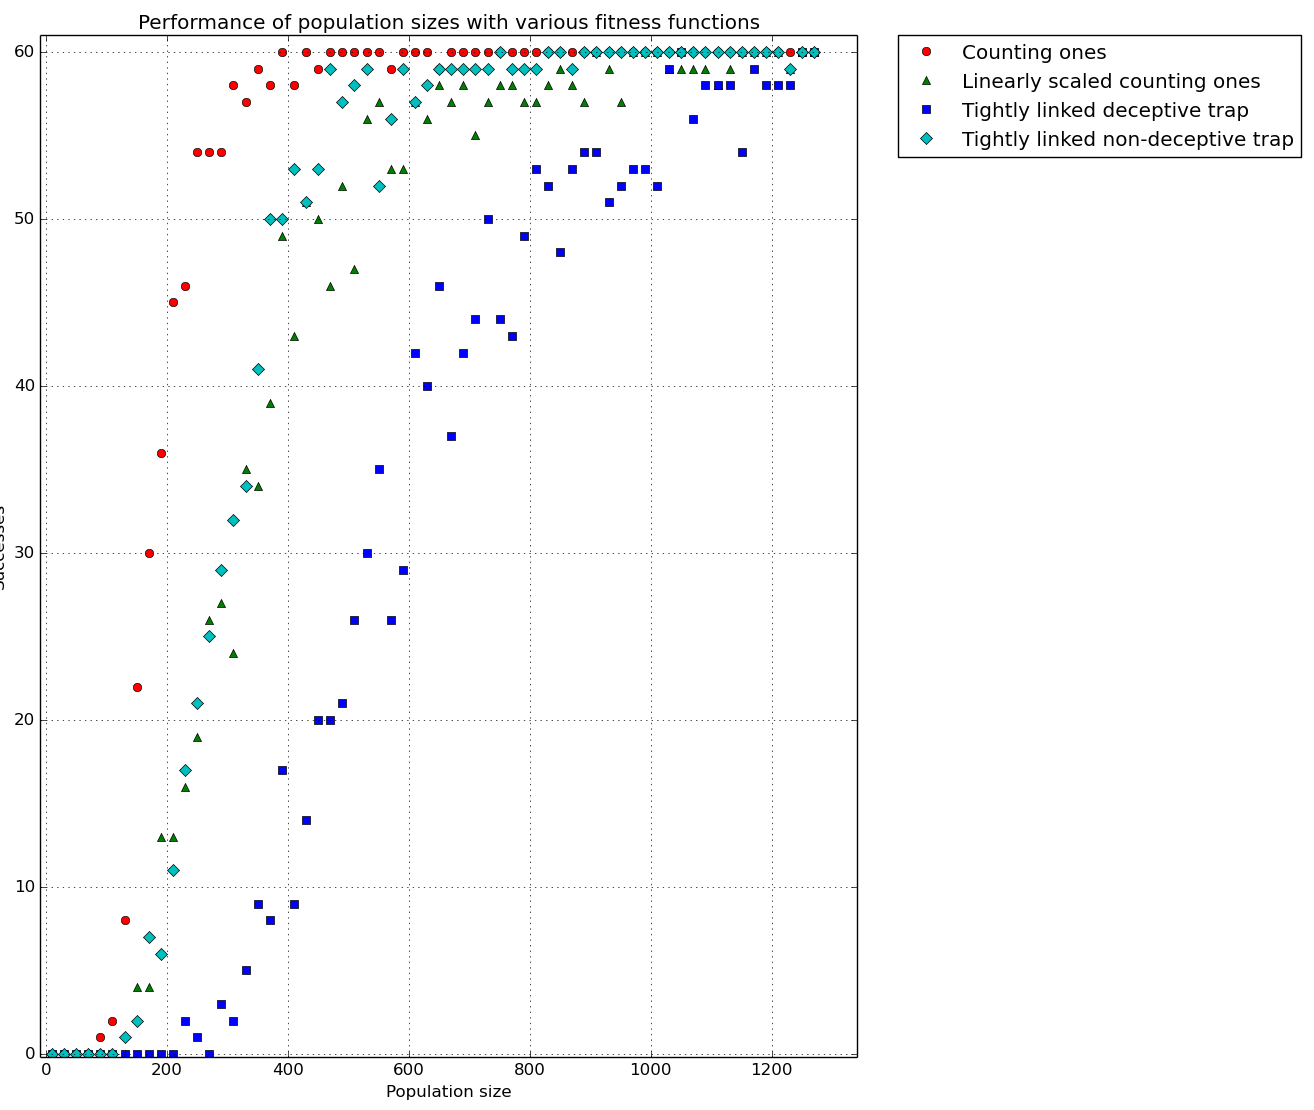
\includegraphics[totalheight=0.7\textheight]{images/exp1.png}
    \caption{Number of success per population size}
\label{fig:exp1}
\end{figure}

\begin{table}[!htb]
\begin{adjustwidth}{0cm}{}
\centering
\begin{tabular}{lp{2.5cm}p{2.5cm}p{2.8cm}}
\toprule[1.5pt]
\bf Fitness function & \bf Population size & \bf Function evaluations & \bf Corresponding CPU time\\\midrule
Counting ones & 310 & 51094 & 0.013 seconds \\
Linearly scaled Counting ones & 730 & 164174 & 0.030 seconds \\
Tightly linked deceptive trap & 1210 & 243142 & 0.429 seconds \\
Tightly linked non-deceptive trap & 610 & 93278 & 0.177 seconds \\
\bottomrule[1.25pt]
\end{tabular}\par
\bigskip
\captionof{table}{Fitness function evaluations}
\label{tab:exp1}
\end{adjustwidth}
\end{table}

% Constructs: to be expected, intuitively clear, not surprising, evident
\paragraph{Observations}
% two-point crossover is bad for randomly linked trap functions
The first observation one can make is that randomly linked trap functions never reach an optimum with population sizes lower than 1280.
This is not surprising since the two-point crossover can't flip multiple bits
in random places at the same time, which is important to improve subfunctions to their best state.
Unless the optimum is generated by accident at a very early stage of the evolution
(the probability of this happening is very small for the population sizes we've tried),
0s will soon dominate a lot of bit positions.
Since the two point crossover can't turn them into ones, an optimum will never be found.

% TODO: maybe mention that if a group of 4 bits are not all ones at an early stage,
% they will all converge to zero.
% The probability of a group of 4 being all 1 at once is not so big.
% The probability of every group of 4 being all 1 in at least one good state in the population
% is apparently very small
% Maybe compute this probability

% two-point crossover is okay for co and lsco
We can also see that \co{} needs the smallest population size.
This is to be expected, because if two parents have many 1s,
their offspring is also very likely to have many 1s.
And since all bits are awarded equally, it is very likely that at every stage of the evolution,
every bit position has a 1 in some member of the population, even if the population is small.

With similar reasoning it is intuitively clear why the two-point crossover needs a
higher population size with \lsco{} than with \co{}.
With \lsco{} the most significant bits contribute more to the fitness, so states with many 1s
on significant places survive better than states with many ones on insignificant places.
To make sure we don't lose the states that have the insignificant bits set to 1, we need
a population size that is big enough to ensure the diversity of the population,
i.e.\ that every bit position has a 1 in some state in the population.

% two-point crossover is okay for tnt
% two-point crossover is good for structure in general
For \tnt{}, even though all bits in a chunk (a subfunction of 4 bits) have to be turned to 1
at the same time in order to be awarded, the population size that is needed is not so big.
Apparently, bits being 1 are not punished so hard that states with many 1s don't survive.
Instead, presumably the states with many 1s will do well, because all the chunks that
are all 1 simultaneously are awarded so much, they can often compensate for the punishments of
the remaining 1s.
Moreover, the two-point crossover is very capable of inheriting one or more chunks that are
completely set to 1, i.e.\ it is not very disruptive in this case.
Generally, two-point crossover is good when the fitness function is structured such that
bits that are close to each other are often also statistically dependent of each other.
In contrast with this, Experiment~\ref{ssec:exp2} will show that this is not the case for
uniform crossover.

% Reducing deceptiveness works well
Furthermore we can observe that \tdt{} needs a higher population size than \tnt{}.
Chunks that are completely set to 1 are less awarded now,
so states with a many 1s are punished harder on average.
A bigger population is needed here to make sure that the population remains diverse enough,
i.e.\ every bit position has a 1 in at least one member of the population.
From this we could draw the general conclusion that reducing deceptiveness in a fitness function
may significantly reduce the population size needed.

% Profiling, function evaluation CPU time matters
Finally we notice that although \lsco{} had more function evaluations than \tnt{},
the cumulative CPU time used is lower.
So evaluating \lsco{} is faster than \tnt{}.
The profile report also showed that in the end the evolution finished faster as well
(0.108 vs 0.240 seconds).
We can conclude from this that a sophisticated fitness function may perform worse than
a less sophisticated function, even though the number of function evaluations is lower.

% TODO: maybe say something about (time/nr evals) ratio


\section{Second Experiment}
\label{ssec:exp2}
In Figure~\ref{fig:exp2} the number of successes has been plot against the population size.
Table~\ref{tab:exp2} shows information concerning the fitness function evaluations.
Tightly linked deceptive trap never reached an optimum, so that one is not shown.

\begin{figure}[!htb]
    \centering
    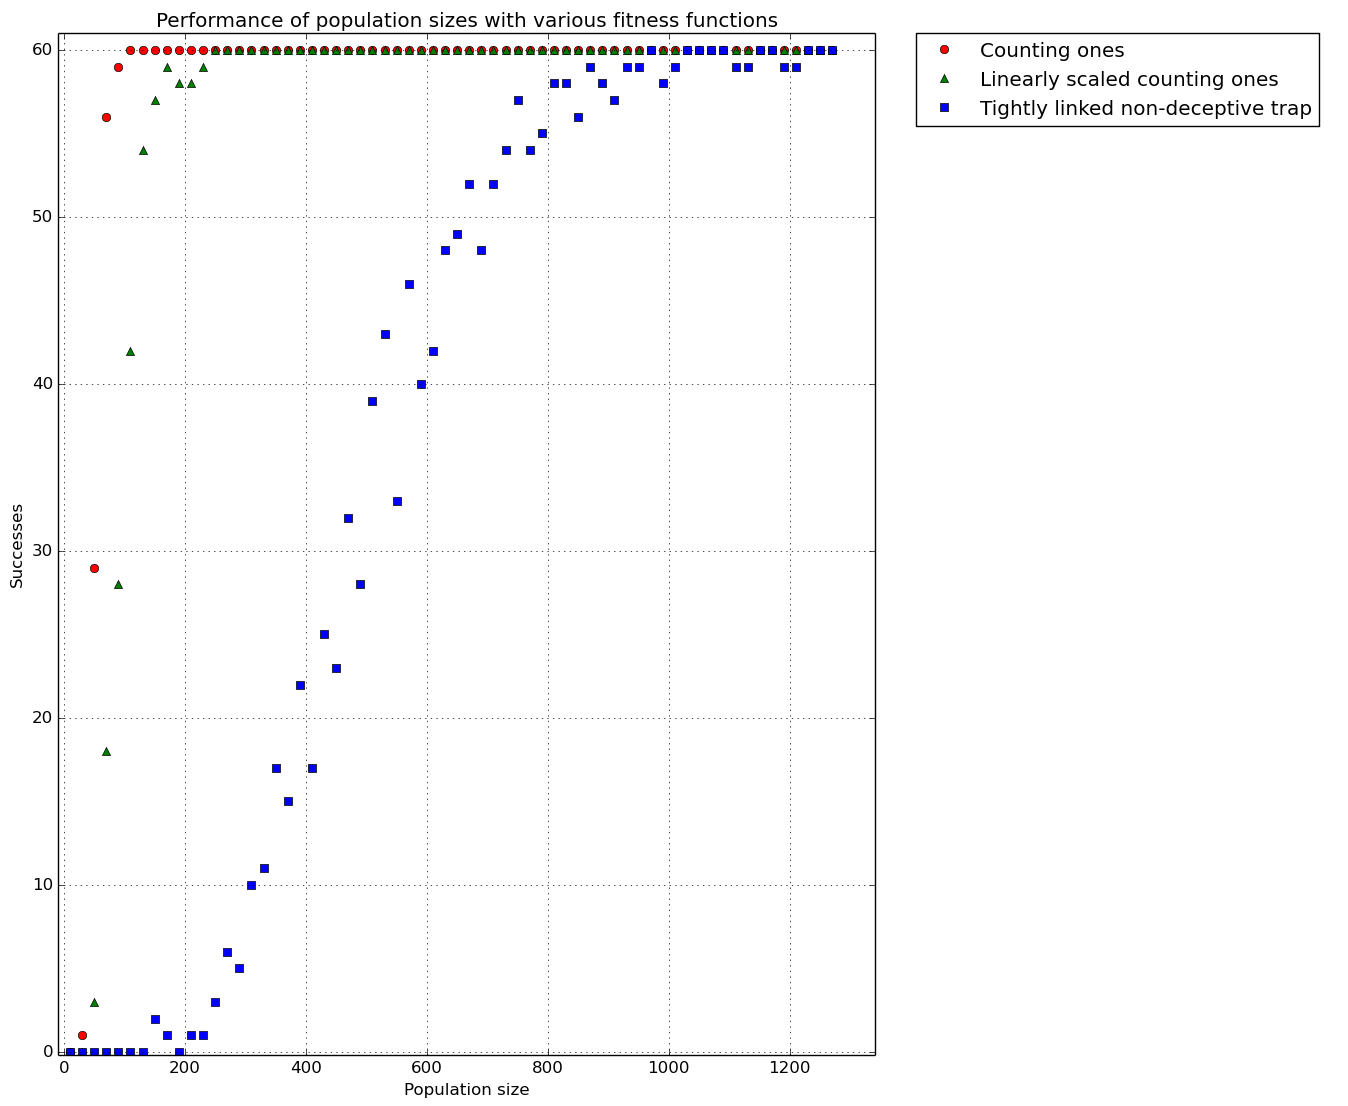
\includegraphics[totalheight=0.7\textheight]{images/exp2.png}
    \caption{Number of success per population size}
\label{fig:exp2}
\end{figure}

\begin{table}[!htb]
\begin{adjustwidth}{0cm}{}
\centering
\begin{tabular}{lp{2.5cm}p{2.5cm}p{2.8cm}}
\toprule[1.5pt]
\bf Fitness function & \bf Population size & \bf Function evaluations & \bf Corresponding CPU time\\\midrule
Counting ones & 70 & 9822 & 0.002 seconds \\
Linearly scaled Counting ones & 160 & 28260 & 0.005 seconds \\
Tightly linked non-deceptive trap & 850 & 242154 & 0.454 seconds \\
\bottomrule[1.25pt]
\end{tabular}\par
\bigskip
\captionof{table}{Fitness function evaluations}
\label{tab:exp2}
\end{adjustwidth}
\end{table}

\paragraph{Observations}
% Two point crossover is better for tightly linked
% Uniform crossover is better for randomly linked, but not perfect
% Ideally, one would like to have a crossover that would capture structure in randomly linked
% Maybe that probabilistic thing would do
The first observation we make is that \tdt{} never reached an optimum.
However, in Experiment~\ref{ssec:exp1} it did.
That makes sense, because the two-point crossover is better for situations with
statistical interaction between bits w.r.t.\ to fitness, whereas uniform crossover doesn't
consider any interaction at all.
Since \tdt{} clearly comprises statistical interaction between bits (bits interact in chunks
of 4 bits), it is not a surprise that uniform crossover needs a larger population size than
two-point crossover to reliably reach the optimum.

We can make a similar observation for \tnt{}, since here the populationsize needed is also
significantly larger than with Experiment~\ref{ssec:exp1}.

% uniform crossover is good for fitness without interconnecting structure
On the other hand, \co{} and \lsco{} need a much smaller population size than in
Experiment~\ref{ssec:exp1}.
This makes sense, because with these fitness functions there is no interaction between bits,
and uniform crossover only looks at individual bits.
% TBC -------------------------------------------------------------------------------------

A final remark we make, is that for the uniform crossover randomly linkedness is the same
as tighly linkedness, since it only looks at individual bits.
Therefore, while it may seem to perform worse on the trap functions, we must not forget
that the uniform crossover solves \rnt{} equivalently as \tnt{}.
So while the two-point crossover could't reach an optimum with \rnt{} at all,
the uniform crossover could.


\section{Third Experiment}
\label{ssec:exp3}
In Figure~\ref{fig:exp3} the number of successes has been plot against the population size.
Table~\ref{tab:exp3} shows information concerning the fitness function evaluations.
Tightly linked deceptive trap never reached an optimum, so it's not shown.

\begin{figure}[!htb]
    \centering
    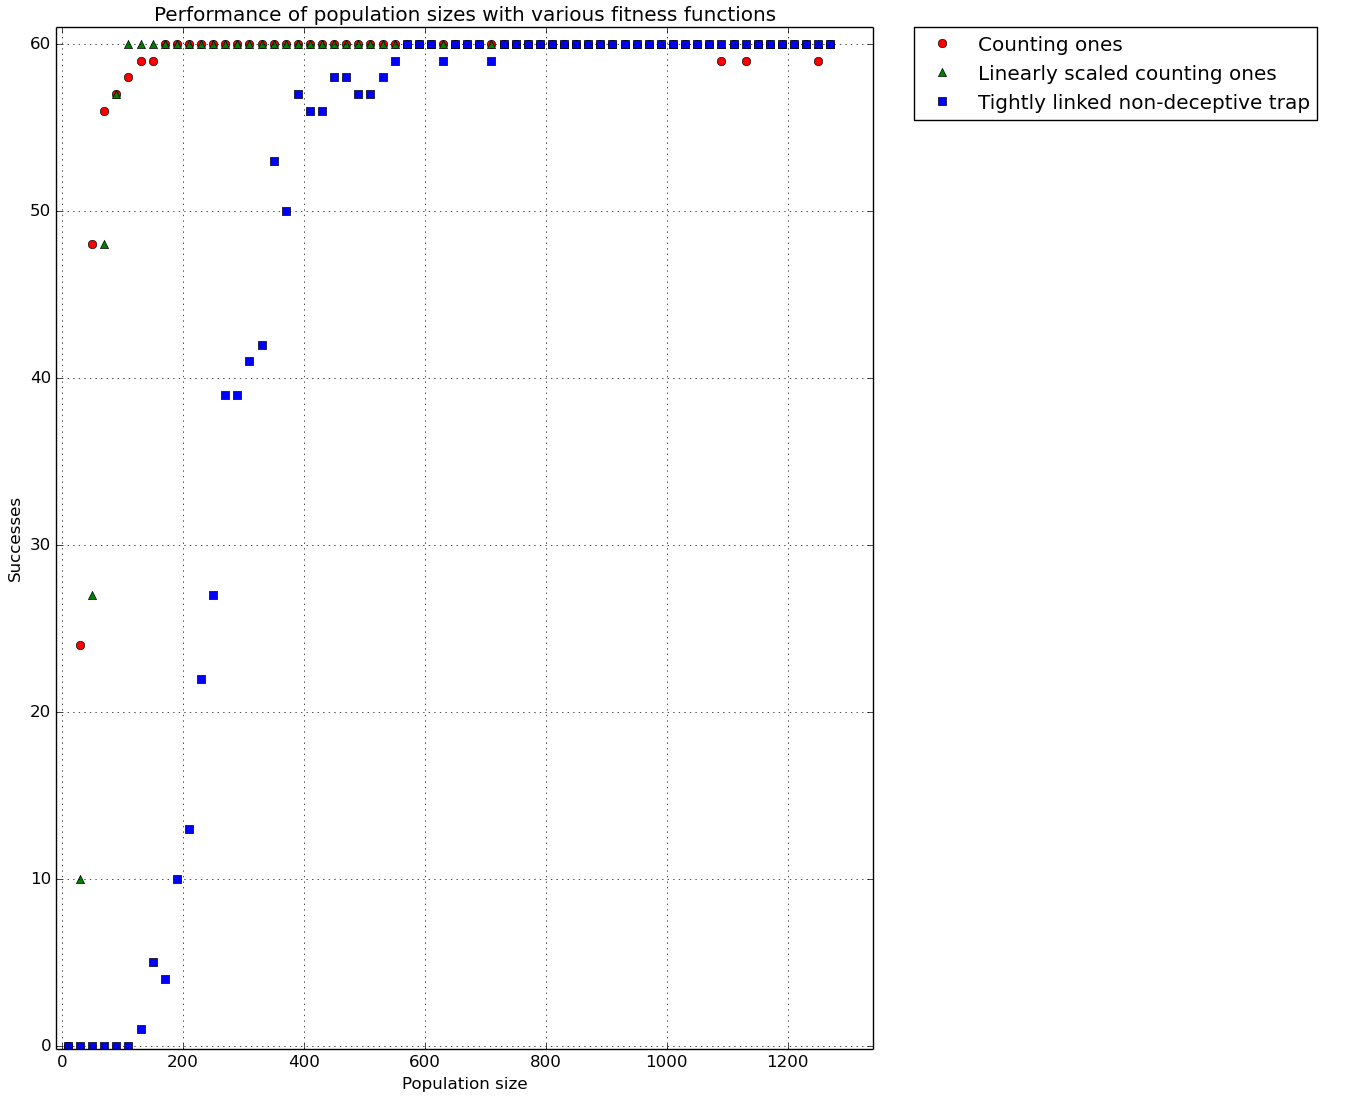
\includegraphics[totalheight=0.7\textheight]{images/exp3.png}
    \caption{Number of success per population size}
\label{fig:exp3}
\end{figure}

\begin{table}[!htb]
\begin{adjustwidth}{0cm}{}
\centering
\begin{tabular}{lp{2.5cm}p{2.5cm}p{2.8cm}}
\toprule[1.5pt]
\bf Fitness function & \bf Population size & \bf Function evaluations & \bf Corresponding CPU time\\\midrule
Counting ones & 110 & 27964 & 0.007 seconds \\
Linearly scaled Counting ones & 90 & 49764 & 0.010 seconds \\
Tightly linked non-deceptive trap & 490 & 509742 & 0.582 seconds \\
\bottomrule[1.25pt]
\end{tabular}\par
\bigskip
\captionof{table}{Fitness function evaluations}
\label{tab:exp3}
\end{adjustwidth}
\end{table}

\paragraph{Observations}
% Mutation helps trap functions
A first observation we can make is that allowing mutation didn't help making \tdt{} find
an optimum with a population size of at most 1280.
A second observation is that it did help to bring down the minimum required population size
for \tnt{} with a factor 2.
% How mutation could bring down the popsize
Seemingly the mutation operator improved the expected diversity of the population by its
disruptive behaviour.
And of course, if for some bit position there were no state in the population with a 1 in there,
the mutation operator gives a possibility to make it appear again.

% Low popsize doesn't mean fast convergence
Another noteworthy observation is that the population size for \lsco{} is about the same
as for \co{}, but that the number of function evaluations is twice as much.
Running a quick test showed that the number of iterations that had to be done before the
evolution finished was also twice as much, which explains the difference.
So while allowing mutation has helped to bring down the population size for \lsco{}
in comparison with Experiment~\ref{ssec:exp2},
it doesn't help to speed up the evolution necessarily, because much more
function evaluations had to be done.


\section*{Final Conclusions}
% What kind of operators are suited for what kind of fitness functions and how this affects
% popsize and CPU time

We can draw several conclusions from the observations we have done in the above sections.

Firstly, two-point crossover is bad for randomly linked trap functions,
since they can't convert multiple bits at random places at the same time.
Two-point crossover is okay for \co{} and \lsco{} and \tnt{}.
In general we can say that the two-point crossover works well if the fitness function is
structured such that bits that are close to each other also comprise some statistical interaction.
So two-point crossover is better for tightly linked trap functions than uniform crossover.

Secondly, if there is a trap in your fitness functions, it may help to try to award the optimum more,
i.e.\ make it non-deceptive, because throughout the experiments we see that the
non-deceptive trap functions requires a significantly smaller population and less CPU time to find
the optimum in comparison with the deceptive trap functions, and never the other way around.

Another lesson we can learn is that a sophisticated fitness function may perform worse than a less sophisticated function.
In Experiment~\ref{ssec:exp1} we saw an example where \tnt{} needed less
function evaluations than \lsco{}, but took a longer time to find the optimum due to its higher
evaluation time.
So even though the number of function evaluations may be less, the total computation time
may be more.

Uniform crossover is better for randomly linked trap functions than two-point crossover,
but still far from perfect.
Ideally, one would like to have a crossover that would capture structure in randomly linked
trap functions.
Maybe a probabilistic model-building approach would be able to do that.
Uniform crossover is good for fitness without interconnecting structure,
therefore it performs well with \co{} and \lsco{}.

Mutation helps to beat trap functions.
In Experiment~\ref{ssec:exp3} we saw that it helped to lower the population size needed.
In general we can say that whenever you have a fitness function that suffers from a
lack of diversity in the population, adding mutation may help increasing the diversity again
through its disruptive behaviour.

Finally, we also saw that a small required population size doesn't necessarily imply
a fast convergence.
Compare \co{} and \lsco{} in Experiment~\ref{ssec:exp3}.

\begin{thebibliography}{9}

\bibitem{cython}
R. Bradshaw, S. Behnel, D. S. Seljebotn, G. Ewing, et al.,
The Cython compiler, \url{http://cython.org}.

\end{thebibliography}


\end{document}
